\documentclass[11pt]{article}

\usepackage[margin=1in]{geometry}
\usepackage[T1]{fontenc}
\usepackage[utf8]{inputenc}
\usepackage{lmodern}
\usepackage{microtype}
\usepackage[table]{xcolor}
\usepackage{amsmath,amssymb,mathtools,bm}
\usepackage{booktabs,array,longtable,tabularx}
\usepackage{hyperref}
\usepackage{enumitem}
\usepackage{fancyhdr}
\usepackage{titlesec}
\usepackage{tcolorbox}
\usepackage{ragged2e}
\usepackage{setspace}
\hypersetup{colorlinks=true,linkcolor=blue!45!black,urlcolor=blue!45!black,citecolor=blue!45!black}
\definecolor{TitleBlue}{HTML}{163A5F}
\definecolor{AccentTeal}{HTML}{2D6F73}
\definecolor{SoftBlue}{HTML}{EAF3F8}
\definecolor{SoftTeal}{HTML}{EDF8F6}
\definecolor{SoftGray}{HTML}{F5F7FA}
\pagestyle{fancy}
\fancyhf{}
\lhead{PINN\_M3DC1}
\rhead{Project Plan}
\cfoot{\thepage}
\fancypagestyle{plain}{%
  \fancyhf{}%
  \lhead{PINN\_M3DC1}%
  \rhead{Project Plan}%
  \cfoot{\thepage}%
}
\setlength{\headheight}{14pt}
\setlength{\parskip}{0.45em}
\setlength{\parindent}{0pt}
\onehalfspacing
\numberwithin{equation}{section}
\titleformat{\section}{\Large\bfseries\color{TitleBlue}}{\thesection}{0.6em}{}
\titleformat{\subsection}{\large\bfseries\color{AccentTeal}}{\thesubsection}{0.6em}{}
\newtcolorbox{overviewbox}{colback=SoftBlue,colframe=TitleBlue,boxrule=0.8pt,arc=2mm,left=3mm,right=3mm,top=2mm,bottom=2mm}
\newtcolorbox{notebox}{colback=SoftGray,colframe=AccentTeal,boxrule=0.6pt,arc=2mm,left=3mm,right=3mm,top=2mm,bottom=2mm}
\newcommand{\DocTitle}[3]{%
\begin{center}
{\LARGE \bfseries \color{TitleBlue} #1}\\[0.5em]
{\large \color{AccentTeal} #2}\\[0.8em]
{\normalsize #3}
\end{center}
\vspace{0.5em}}
\newcommand{\ProjectTOC}{\vspace{0.5em}{\hypersetup{linkcolor=TitleBlue}\tableofcontents}\vspace{0.8em}}
\allowdisplaybreaks

\usepackage{tikz}
\usetikzlibrary{arrows.meta,positioning,calc,decorations.pathreplacing,patterns,shapes.geometric}
\usepackage{caption}
\usepackage{subcaption}
\usepackage{multirow}
\usepackage{makecell}
\usepackage{upquote}

\definecolor{WarningRed}{HTML}{9B2C2C}
\definecolor{WarmGold}{HTML}{B7791F}
\definecolor{PaleGold}{HTML}{FFF8E6}
\definecolor{PaleRed}{HTML}{FFF1F1}
\definecolor{DeepGreen}{HTML}{276749}

\newtcolorbox{definitionbox}[1][]{
  colback=SoftTeal,colframe=AccentTeal,title={Definition#1},
  fonttitle=\bfseries,boxrule=0.7pt,arc=2mm,
  left=3mm,right=3mm,top=2mm,bottom=2mm}
\newtcolorbox{warningbox}[1][]{
  colback=PaleRed,colframe=WarningRed,title={Important distinction#1},
  fonttitle=\bfseries,boxrule=0.7pt,arc=2mm,
  left=3mm,right=3mm,top=2mm,bottom=2mm}
\newtcolorbox{checkpointbox}[1][]{
  colback=PaleGold,colframe=WarmGold,title={Verification checkpoint#1},
  fonttitle=\bfseries,boxrule=0.7pt,arc=2mm,
  left=3mm,right=3mm,top=2mm,bottom=2mm}
\newtcolorbox{conventionbox}[1][]{
  colback=SoftBlue,colframe=TitleBlue,title={Frozen Module 2 convention#1},
  fonttitle=\bfseries,boxrule=0.9pt,arc=2mm,
  left=3mm,right=3mm,top=2mm,bottom=2mm}
\newtcolorbox{resultbox}[1][]{
  colback=SoftTeal,colframe=DeepGreen,title={Required result#1},
  fonttitle=\bfseries,boxrule=0.8pt,arc=2mm,
  left=3mm,right=3mm,top=2mm,bottom=2mm}

\newcommand{\dd}{\mathrm{d}}
\newcommand{\pd}{\partial}
\newcommand{\vect}[1]{\bm{#1}}
\newcommand{\bracket}[2]{\left[#1,#2\right]}
\newcommand{\average}[1]{\left\langle #1\right\rangle}
\newcommand{\Lap}{\nabla_{\!\perp}^{2}}
\newcommand{\F}{\mathcal{F}}
\newcommand{\InvF}{\mathcal{F}^{-1}}
\newcommand{\norm}[1]{\left\lVert #1\right\rVert}

\pagestyle{fancy}
\fancyhf{}
\lhead{PINN\_M3DC1}
\rhead{Module 2 Physics Notes}
\cfoot{\thepage}
\fancypagestyle{plain}{%
  \fancyhf{}%
  \lhead{PINN\_M3DC1}%
  \rhead{Module 2 Physics Notes}%
  \cfoot{\thepage}%
}

\begin{document}
\hypersetup{pageanchor=false}

\begin{titlepage}
\centering
\vspace*{1.15cm}
{\Large\color{AccentTeal} PINN\_M3DC1}\par
\vspace{0.7cm}
{\Huge\bfseries\color{TitleBlue} Module 2}\par
\vspace{0.25cm}
{\LARGE\bfseries\color{TitleBlue} Synthetic MHD Solver\\and Case Generation}\par
\vspace{0.9cm}
{\large A textbook-style numerical-physics specification for periodic magnetic-island coalescence}\par
\vfill
\begin{tcolorbox}[width=0.90\textwidth,colback=SoftBlue,colframe=TitleBlue,arc=2mm]
\centering
\textbf{Module purpose}\par
\vspace{0.35em}
Generate reproducible, verified trajectories of a two-dimensional reduced resistive-MHD island-coalescence problem, together with spatial and temporal convergence evidence suitable for later surrogate learning.
\end{tcolorbox}
\vfill
{\normalsize Version 1.0 \quad | \quad 5 August 2026}\par
\vspace{0.25cm}
{\small Physics and numerical-method note for the synthetic reduced-MHD proof of concept}\par
\end{titlepage}

\hypersetup{pageanchor=true}
\pagenumbering{roman}

\section*{Preface: what Module 2 must establish}

Module~1 defined the physical model. Module~2 must now answer a different question: how do we turn those continuous partial differential equations into trustworthy numerical trajectories?

That question cannot be answered by producing an attractive animation. A numerical field can look smooth and plausible while containing a sign error, an aliased nonlinear term, a poorly resolved current sheet, an unstable time step, or a false reconnection event caused by numerical diffusion. Because the later neural networks learn from these fields, every systematic solver error becomes part of the training target. Module~2 is therefore the scientific foundation beneath Modules~3--6.

The initials \textbf{MHD} mean \emph{magnetohydrodynamics}. A \textbf{synthetic case} is a numerical trajectory generated by the reduced model selected by this project, rather than an experimental measurement or a genuine M3D-C1 calculation. A \textbf{pseudo-spectral method} represents periodic fields by Fourier modes, differentiates those modes algebraically, and evaluates nonlinear products on a physical grid. A \textbf{convergence study} demonstrates that selected numerical answers approach a stable limit when the spatial and temporal discretizations are refined.

\begin{warningbox}
The word \emph{synthetic} does not mean arbitrary or unverified. It means that the data are generated by the stated two-field reduced-MHD initial-value problem. These data can support a reduced-MHD surrogate proof of concept. They cannot, by themselves, support a claim of fidelity to M3D-C1.
\end{warningbox}

\subsection*{How to read this note}

The main dependency chain is
\[
\begin{gathered}
\text{frozen reduced-MHD equations}
\longrightarrow \text{periodic initial-value problem}
\longrightarrow \text{Fourier representation}\\
\longrightarrow \text{dealiased nonlinear evaluation}
\longrightarrow \text{time integration}
\longrightarrow \text{diagnostics}\\
\longrightarrow \text{verification and convergence}
\longrightarrow \text{accepted HDF5 trajectory}.
\end{gathered}
\]
Sections~\ref{sec:role}--\ref{sec:initial} define the exact physical case. Sections~\ref{sec:fourier}--\ref{sec:time} derive the numerical method. Sections~\ref{sec:diagnostics}--\ref{sec:convergence} define the evidence required before a trajectory is accepted. Sections~\ref{sec:generation}--\ref{sec:contract} freeze the case-generation and implementation contracts. The appendices collect derivations, symbols, terminology, and concept questions.

\subsection*{Learning objectives}

After working through this module, the reader should be able to:
\begin{enumerate}[label=\arabic*.]
  \item distinguish a mathematical solution, a numerical approximation, a stored trajectory, and a rendered plot;
  \item state exactly which fields the solver advances and which fields it reconstructs;
  \item derive the periodic island-coalescence initial fields and locate their O-points and X-points;
  \item explain why the unperturbed magnetic array is an equilibrium of the ideal nonlinear equations;
  \item explain how the stream-function perturbation drives two parallel current channels together;
  \item represent a periodic field by discrete Fourier coefficients and differentiate it spectrally;
  \item invert $\Lap U=\omega$ while treating the zero Fourier mode correctly;
  \item explain how a pseudo-spectral method differs from a fully spectral Galerkin method;
  \item derive the Fourier-space right-hand sides for $\psi$ and $\omega$;
  \item explain aliasing and apply the two-thirds truncation rule;
  \item implement one classical fourth-order Runge--Kutta step without using stale derived fields;
  \item monitor advective, Alfv\'enic, and diffusive time-step restrictions;
  \item define energy, current-sheet, symmetry, topology, and reconnection diagnostics;
  \item distinguish code verification from model validation;
  \item conduct separate temporal and spatial refinement studies;
  \item calculate observed convergence order and self-convergence error;
  \item decide whether a current sheet is resolved using spectra and physical-space measures;
  \item define a reproducible parameter sweep without accepting unconverged cases;
  \item identify the metadata required to reproduce a stored trajectory; and
  \item state precisely what evidence Module~2 does and does not provide.
\end{enumerate}

\ProjectTOC
\clearpage
\pagenumbering{arabic}

\section{Scientific role and acceptance boundary}
\label{sec:role}

\subsection{The numerical object being built}

For a fixed parameter vector
\begin{equation}
\vect{\mu}=(\eta,\nu,A_0),
\end{equation}
the solver approximates a trajectory
\begin{equation}
\mathcal{Q}_{\vect{\mu}}
=\left\{\psi(x,y,t),U(x,y,t),J(x,y,t),\omega(x,y,t):
(x,y)\in\Omega,\ 0\le t\le T\right\}.
\end{equation}
Here $\eta$ is magnetic diffusivity, $\nu$ is kinematic viscosity, and $A_0$ is the amplitude of the initial flow perturbation. All three are dimensionless under the physical normalization frozen in Module~1.

The mathematical state is continuous. A computed case is finite:
\begin{equation}
\mathcal{Q}^{N_x,N_y,\Delta t}_{\vect{\mu}}
=\left\{\psi_{ijn},U_{ijn},J_{ijn},\omega_{ijn}\right\},
\end{equation}
where $i$ and $j$ label grid points and $n$ labels saved times. The superscripts emphasize that the stored result depends on resolution and time step. The convergence program must show that this dependence is acceptably small for the quantities used later.

\subsection{Four levels of evidence}

\begin{longtable}{p{0.18\textwidth}p{0.34\textwidth}p{0.38\textwidth}}
\toprule
Level & Question & Required evidence \\
\midrule
\endfirsthead
\toprule
Level & Question & Required evidence \\
\midrule
\endhead
Definition & Is the intended problem unambiguous? & Equations, signs, initial conditions, periodicity, gauges, parameters, and diagnostics are frozen. \\
Verification & Does the code solve those equations correctly? & Exact modes, manufactured solutions, operator tests, balance laws, parity, and convergence. \\
Numerical adequacy & Is this particular nonlinear trajectory resolved? & Spectral tails, current-sheet resolution, stable diagnostics, and refinement agreement. \\
Validation & Does the reduced model represent a target physical system or M3D-C1? & External observations or genuine higher-fidelity calculations. This evidence is not produced by Module~2. \\
\bottomrule
\end{longtable}

\begin{definitionbox}
\textbf{Verification} asks whether the equations were solved correctly. \textbf{Validation} asks whether the chosen equations represent the physical target adequately. A code can be verified for a reduced model without that reduced model being validated as a substitute for M3D-C1.
\end{definitionbox}

\subsection{Module 2 deliverables}

Module~2 is complete only when the project can produce:
\begin{enumerate}[label=\arabic*.]
  \item an independently reproducible Python trajectory;
  \item an independently reproducible MATLAB trajectory using the same mathematical contract;
  \item a baseline island-coalescence case with complete metadata;
  \item an exact-mode or manufactured-solution verification report;
  \item a temporal-refinement report;
  \item a spatial-refinement and spectral-resolution report;
  \item energy, mean, periodicity, divergence, symmetry, and topology histories;
  \item Python--MATLAB parity metrics on a common saved grid; and
  \item a case manifest that records whether every acceptance criterion passed.
\end{enumerate}

\begin{resultbox}
A single contour plot is not a Module~2 deliverable. The accepted object is a numerical field trajectory plus enough evidence and metadata for another implementation to reproduce and audit it.
\end{resultbox}

\section{Frozen reduced-MHD initial-value problem}
\label{sec:ivp}

\subsection{Domain and periodicity}

The version-1 domain is the half-open square
\begin{equation}
\Omega=[0,L_x)\times[0,L_y),
\qquad L_x=L_y=2\pi.
\label{eq:domain}
\end{equation}
The half-open notation means that $x=0$ is stored but $x=2\pi$ is not stored; those positions are the same periodic point. The same convention applies in $y$.

For every field and every derivative needed by the equations,
\begin{align}
f(x+2\pi,y,t)&=f(x,y,t),\\
f(x,y+2\pi,t)&=f(x,y,t).
\end{align}
Fourier representation enforces this smooth periodic structure by construction.

\subsection{Fields and signs}

The primary physical fields are the magnetic-flux function $\psi$ and flow stream function $U$. The frozen Module~1 definitions are
\begin{align}
\vect{B}_{\perp}
&=\nabla\psi\times\widehat{\vect{z}}
=(\psi_y,-\psi_x),\\
\vect{v}_{\perp}
&=\widehat{\vect{z}}\times\nabla U
=(-U_y,U_x),\\
J&=-\Lap\psi,\\
\omega&=\Lap U,\\
\bracket{f}{g}
&=f_xg_y-f_yg_x.
\end{align}
Consequently,
\begin{equation}
\bracket{U}{f}=\vect{v}_{\perp}\cdot\nabla f.
\end{equation}

\subsection{Evolution equations}

The solver advances
\begin{align}
\pd_t\psi+\bracket{U}{\psi}
&=\eta\Lap\psi,
\label{eq:psi}\\
\pd_t\omega+\bracket{U}{\omega}
&=\bracket{J}{\psi}+\nu\Lap\omega,
\label{eq:omega}\\
J&=-\Lap\psi,
\qquad
\omega=\Lap U.
\label{eq:definitions}
\end{align}
Equivalently,
\begin{align}
\pd_t\psi
&=-\bracket{U}{\psi}-\eta J,\\
\pd_t\omega
&=-\bracket{U}{\omega}+\bracket{J}{\psi}+\nu\Lap\omega.
\end{align}

The solver's most convenient prognostic variables are $(\psi,\omega)$. At every time-integration stage it reconstructs $U$ from $\Lap U=\omega$ and derives $J=-\Lap\psi$. The stored dataset fields remain $(\psi,U,J,\omega)$.

\begin{conventionbox}
The code must never advance four independent arrays for $\psi$, $U$, $J$, and $\omega$. Doing so would permit violations of $J=-\Lap\psi$ and $\omega=\Lap U$. Advance $(\psi,\omega)$, reconstruct $(U,J)$ at every stage, and store all four only after their definitions agree.
\end{conventionbox}

\subsection{Gauge and zero-mode constraints}

Only derivatives of $U$ affect the physical velocity, so
\begin{equation}
\average{U}(t)=0
\end{equation}
fixes its arbitrary additive constant. The initial flux has zero mean, and the periodic equation preserves
\begin{equation}
\average{\psi}(t)=0.
\end{equation}
Because $J$ and $\omega$ are periodic Laplacians,
\begin{equation}
\average{J}=\average{\omega}=0.
\end{equation}
These are exact compatibility conditions. They should be enforced at the zero Fourier mode and monitored in physical space.

\subsection{Total-energy identity}

The magnetic, kinetic, and total energies are
\begin{align}
E_B(t)&=\frac12\int_\Omega|\nabla\psi|^2\,\dd A,\\
E_K(t)&=\frac12\int_\Omega|\nabla U|^2\,\dd A,\\
E(t)&=E_B(t)+E_K(t).
\end{align}
Smooth periodic solutions satisfy
\begin{equation}
\boxed{
\frac{\dd E}{\dd t}
=-\eta\int_\Omega J^2\,\dd A
-\nu\int_\Omega\omega^2\,\dd A.}
\label{eq:energy}
\end{equation}
This identity is the principal global sign and dissipation audit, but it is not sufficient by itself: many wrong fields can share a similar energy history.

\section{The periodic island-coalescence benchmark}
\label{sec:initial}

\subsection{Why island coalescence is useful}

Two parallel current channels attract magnetically. In a two-dimensional flux map, each channel sits inside a magnetic island. The islands move toward one another, compress the field between them, form a thin current sheet near an X-point, and reconnect at finite resistivity. This single case exercises all important version-1 terms:
\begin{itemize}
  \item flux advection $\bracket{U}{\psi}$;
  \item vorticity advection $\bracket{U}{\omega}$;
  \item Lorentz forcing $\bracket{J}{\psi}$;
  \item resistive diffusion $\eta\Lap\psi$;
  \item viscous diffusion $\nu\Lap\omega$;
  \item nonlinear transfer between magnetic and kinetic energy;
  \item current-sheet formation; and
  \item resistive change of magnetic topology.
\end{itemize}

The benchmark is adapted to the project's $[0,2\pi)^2$ coordinates and sign conventions from the classical periodic coalescence problem used by Ng and collaborators \cite{Ng2008,Ng2011}.

\subsection{Exact initial fields}

The fixed equilibrium amplitude is
\begin{equation}
\Psi_{\rm eq}=1.
\end{equation}
The version-1 initial condition is
\begin{align}
\psi(x,y,0)
&=\psi_0(x,y)
=\Psi_{\rm eq}\sin x\sin y,
\label{eq:psi0}\\
U(x,y,0)
&=U_0(x,y)
=A_0(\cos x-\cos y).
\label{eq:U0}
\end{align}
The parameter $A_0\ge0$ controls the coalescence-driving flow. The corresponding derived fields are
\begin{align}
J_0
&=-\Lap\psi_0
=2\Psi_{\rm eq}\sin x\sin y
=2\psi_0,
\label{eq:J0}\\
\omega_0
&=\Lap U_0
=-A_0(\cos x-\cos y)
=-U_0,
\label{eq:omega0}\\
\vect{B}_{\perp,0}
&=\Psi_{\rm eq}(\sin x\cos y,-\cos x\sin y),
\label{eq:B0}\\
\vect{v}_{\perp,0}
&=(-A_0\sin y,-A_0\sin x).
\label{eq:v0}
\end{align}

\begin{checkpointbox}
Equations~\eqref{eq:J0} and \eqref{eq:omega0} are immediate sign tests. If an implementation produces $J_0=-2\psi_0$ or $\omega_0=+U_0$, its Fourier Laplacian or frozen field convention is wrong.
\end{checkpointbox}

\subsection{Why the magnetic array is an equilibrium}

Set $A_0=0$, so $U_0=\omega_0=0$. Because
\begin{equation}
J_0=2\psi_0,
\end{equation}
the Lorentz bracket vanishes:
\begin{equation}
\bracket{J_0}{\psi_0}
=\bracket{2\psi_0}{\psi_0}=0.
\end{equation}
Thus the initial magnetic field produces no vorticity forcing in the ideal two-field model. When $\eta=0$, it is a static exact equilibrium.

At finite $\eta$ and $A_0=0$, the shape remains a single Fourier eigenmode:
\begin{align}
\psi_{\rm exact}(x,y,t)
&=\Psi_{\rm eq}e^{-2\eta t}\sin x\sin y,\\
U_{\rm exact}(x,y,t)&=0,\\
J_{\rm exact}(x,y,t)&=2\psi_{\rm exact},\\
\omega_{\rm exact}(x,y,t)&=0.
\label{eq:exactdecay}
\end{align}
This exact resistively decaying solution is one of the strongest Module~2 verification cases.

\subsection{O-points, X-points, and current channels}

The magnetic critical points satisfy $\nabla\psi_0=0$. The four island centers in one fundamental domain are
\begin{center}
\begin{tabular}{cccc}
\toprule
Point & Coordinate & $\psi_0/\Psi_{\rm eq}$ & $J_0/\Psi_{\rm eq}$ \\
\midrule
$O_{++}^{(1)}$ & $(\pi/2,\pi/2)$ & $+1$ & $+2$ \\
$O_{--}^{(1)}$ & $(\pi/2,3\pi/2)$ & $-1$ & $-2$ \\
$O_{--}^{(2)}$ & $(3\pi/2,\pi/2)$ & $-1$ & $-2$ \\
$O_{++}^{(2)}$ & $(3\pi/2,3\pi/2)$ & $+1$ & $+2$ \\
\bottomrule
\end{tabular}
\end{center}
The points $(m\pi,n\pi)$ are X-points, with integers $m,n$. In particular,
\begin{equation}
X_c=(\pi,\pi)
\end{equation}
lies between the two negative-current islands that the selected perturbation drives together.

\begin{figure}[htbp]
\centering
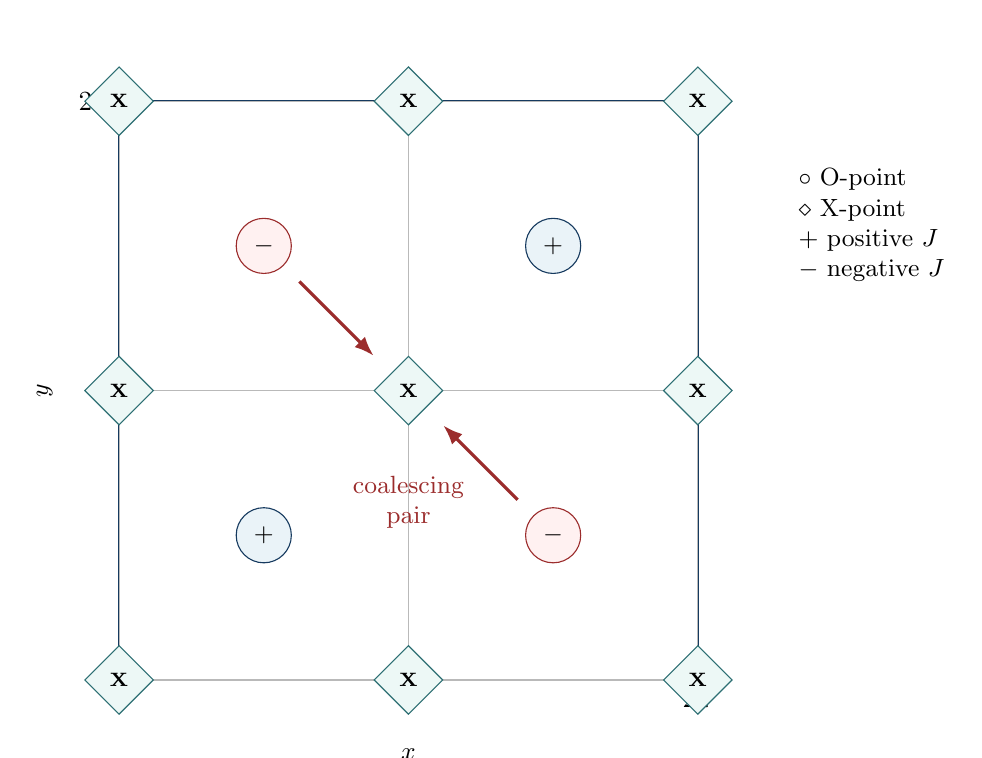
\begin{tikzpicture}[scale=1.05,
  op/.style={circle,draw=TitleBlue,fill=SoftBlue,minimum size=7mm,font=\small\bfseries},
  on/.style={circle,draw=WarningRed,fill=PaleRed,minimum size=7mm,font=\small\bfseries},
  xp/.style={diamond,draw=AccentTeal,fill=SoftTeal,minimum size=6mm,font=\scriptsize\bfseries},
  arr/.style={-{Latex[length=2.5mm]},very thick,color=WarningRed}]
\draw[thick,TitleBlue] (0,0) rectangle (7,7);
\foreach \x/\lab in {0/0,3.5/\pi,7/2\pi}{
  \draw[gray!55] (\x,0)--(\x,7);
  \node[below] at (\x,0) {$\lab$};
}
\foreach \y/\lab in {0/0,3.5/\pi,7/2\pi}{
  \draw[gray!55] (0,\y)--(7,\y);
  \node[left] at (0,\y) {$\lab$};
}
\node[op] at (1.75,1.75) {$+$};
\node[on] at (1.75,5.25) {$-$};
\node[on] at (5.25,1.75) {$-$};
\node[op] at (5.25,5.25) {$+$};
\foreach \x in {0,3.5,7}{
  \foreach \y in {0,3.5,7}{
    \node[xp] at (\x,\y) {X};
  }
}
\draw[arr] (2.18,4.82)--(3.08,3.92);
\draw[arr] (4.82,2.18)--(3.92,3.08);
\node[align=center,font=\small,text=WarningRed] at (3.5,2.15) {coalescing\\pair};
\node[align=left,font=\small] at (9.1,5.5) {$\circ$ O-point\\$\diamond$ X-point\\$+$ positive $J$\\$-$ negative $J$};
\node[font=\small,align=center] at (3.5,-0.9) {$x$};
\node[font=\small,rotate=90] at (-0.9,3.5) {$y$};
\end{tikzpicture}
\caption{Topology of $\psi_0=\sin x\sin y$. The stream-function perturbation drives the two negative-current islands toward the central X-point. Periodicity creates an equivalent pairing of the positive-current islands across the domain boundary. The drawing identifies critical points; it is not a computed trajectory.}
\label{fig:islands}
\end{figure}

\subsection{How the perturbation drives coalescence}

Evaluate Eq.~\eqref{eq:v0} at the two negative-current O-points:
\begin{align}
\vect{v}_{\perp,0}\left(\frac{\pi}{2},\frac{3\pi}{2}\right)
&=(+A_0,-A_0),\\
\vect{v}_{\perp,0}\left(\frac{3\pi}{2},\frac{\pi}{2}\right)
&=(-A_0,+A_0).
\end{align}
Both velocities point toward $(\pi,\pi)$. Since both islands carry current in the same out-of-plane direction, the perturbation selects the attractive coalescence mode. The initial flow is not a random disturbance; its symmetry determines which pair merges inside the displayed fundamental cell.

The early qualitative sequence is
\[
\begin{aligned}
\text{two parallel current channels}
&\longrightarrow \text{approach}\\
&\longrightarrow \text{magnetic compression at }X_c\\
&\longrightarrow \text{thin current sheet}\\
&\longrightarrow \text{finite }\eta\text{ changes }\psi\\
&\longrightarrow \text{reconnected flux and merged topology}.
\end{aligned}
\]

\subsection{Symmetries as diagnostics}

The analytic initial fields have reflection and exchange symmetries. Examples include
\begin{align}
\psi_0(x,y)&=\psi_0(y,x),\\
U_0(x,y)&=-U_0(y,x),\\
\psi_0(2\pi-x,2\pi-y)&=\psi_0(x,y),\\
U_0(2\pi-x,2\pi-y)&=U_0(x,y).
\end{align}
The continuous equations preserve the compatible symmetry class. The solver does not need to impose these relations, but their defects reveal asymmetry from indexing, roundoff amplification, unequal grid treatment, or programming errors.

\subsection{Baseline parameters and time horizon}

The recommended baseline is
\begin{equation}
(\eta,\nu,A_0)=(10^{-3},10^{-3},0.1),
\qquad \Psi_{\rm eq}=1.
\label{eq:baselineparams}
\end{equation}
The principal grid and output settings are
\begin{equation}
N_x=N_y=128,\qquad
\Delta t=10^{-3},\qquad
\Delta t_{\rm save}=0.05.
\end{equation}

The first pilot window is $0\le t\le5$. The accepted coalescence trajectory must extend through the first resolved current or reconnection-rate peak and include a post-peak interval. A nominal production horizon of $T=8$ is therefore used for the baseline unless the convergence pilot demonstrates that a different common horizon is required.

\begin{warningbox}[\,: endpoint]
A final time is not physically adequate merely because the code reached it. If $|J|_{\max}$ and the reconnection rate are still rising at the last snapshot, the run has captured current-sheet formation but not the first coalescence event. Extend the horizon and version the configuration before generating the learning dataset.
\end{warningbox}

\section{Why a Fourier pseudo-spectral method}
\label{sec:fourier}

\subsection{Periodic Fourier basis}

A smooth doubly periodic field can be written
\begin{equation}
f(x,y,t)=
\sum_{m=-\infty}^{\infty}
\sum_{n=-\infty}^{\infty}
\widehat f_{mn}(t)
e^{i(k_{x,m}x+k_{y,n}y)},
\end{equation}
where
\begin{equation}
k_{x,m}=\frac{2\pi m}{L_x},
\qquad
k_{y,n}=\frac{2\pi n}{L_y}.
\end{equation}
For $L_x=L_y=2\pi$, the wave numbers are integers:
\begin{equation}
k_{x,m}=m,\qquad k_{y,n}=n.
\end{equation}

Spectral differentiation follows from
\begin{align}
\pd_x e^{i(k_xx+k_yy)}
&=ik_xe^{i(k_xx+k_yy)},\\
\pd_y e^{i(k_xx+k_yy)}
&=ik_ye^{i(k_xx+k_yy)},\\
\Lap e^{i(k_xx+k_yy)}
&=-(k_x^2+k_y^2)e^{i(k_xx+k_yy)}.
\end{align}
Thus
\begin{align}
\widehat{f_x}_{mn}&=ik_{x,m}\widehat f_{mn},\\
\widehat{f_y}_{mn}&=ik_{y,n}\widehat f_{mn},\\
\widehat{\Lap f}_{mn}&=-k_{mn}^2\widehat f_{mn},
\end{align}
where $k_{mn}^2=k_{x,m}^2+k_{y,n}^2$.

\subsection{Discrete grid and transform}

For even $N_x,N_y$, the collocation grid is
\begin{align}
x_j&=\frac{jL_x}{N_x},
&&j=0,\ldots,N_x-1,\\
y_\ell&=\frac{\ell L_y}{N_y},
&&\ell=0,\ldots,N_y-1.
\end{align}
No duplicated endpoint is stored.

With the common unnormalized forward transform,
\begin{align}
\widehat f_{mn}
&=\sum_{j=0}^{N_x-1}\sum_{\ell=0}^{N_y-1}
f_{j\ell}
e^{-2\pi i(mj/N_x+n\ell/N_y)},\\
f_{j\ell}
&=\frac{1}{N_xN_y}
\sum_{m=0}^{N_x-1}\sum_{n=0}^{N_y-1}
\widehat f_{mn}
e^{2\pi i(mj/N_x+n\ell/N_y)}.
\end{align}
This is the default normalization used by both NumPy's \texttt{fft2}/\texttt{ifft2} and MATLAB's \texttt{fft2}/\texttt{ifft2}. The stored wave-number ordering must follow the actual library ordering, including negative frequencies in the upper index range.

\subsection{Why the method is called pseudo-spectral}

Linear derivatives are evaluated in Fourier space. A nonlinear bracket, however, is evaluated by:
\begin{enumerate}[label=\arabic*.]
  \item multiplying Fourier coefficients by $ik_x$ or $ik_y$;
  \item inverse transforming the derivatives to the physical grid;
  \item multiplying physical-space arrays pointwise; and
  \item transforming the product back to Fourier space.
\end{enumerate}
The method is called \emph{pseudo-spectral} because nonlinear products are evaluated at collocation points rather than by an explicit exact convolution sum over Fourier coefficients.

\begin{figure}[htbp]
\centering
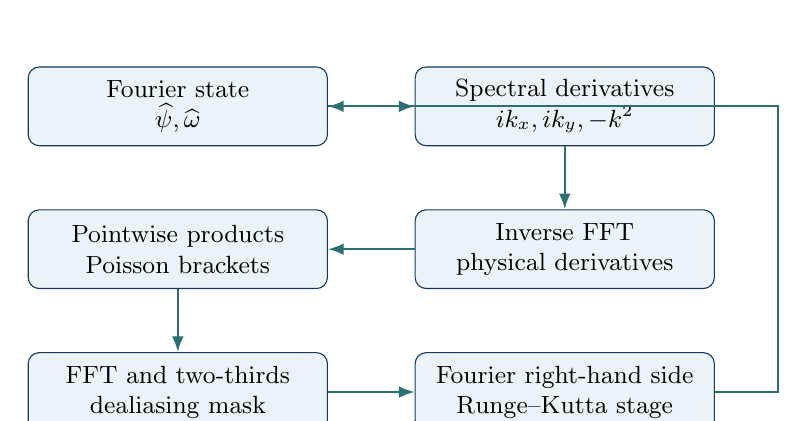
\begin{tikzpicture}[
  node distance=8mm and 11mm,
  box/.style={draw=TitleBlue,rounded corners,fill=SoftBlue,minimum width=3.8cm,minimum height=1.0cm,align=center,font=\small},
  arr/.style={-{Latex[length=2mm]},thick,color=AccentTeal}
]
\node[box] (state) {Fourier state\\$\widehat\psi,\widehat\omega$};
\node[box,right=of state] (derive) {Spectral derivatives\\$ik_x,ik_y,-k^2$};
\node[box,below=of derive] (physical) {Inverse FFT\\physical derivatives};
\node[box,left=of physical] (product) {Pointwise products\\Poisson brackets};
\node[box,below=of product] (filter) {FFT and two-thirds\\dealiasing mask};
\node[box,right=of filter] (rhs) {Fourier right-hand side\\Runge--Kutta stage};
\draw[arr] (state)--(derive);
\draw[arr] (derive)--(physical);
\draw[arr] (physical)--(product);
\draw[arr] (product)--(filter);
\draw[arr] (filter)--(rhs);
\draw[arr] (rhs.east) -- ++(0.8,0) |- (state.east);
\end{tikzpicture}
\caption{One right-hand-side evaluation in the Fourier pseudo-spectral solver. Derived fields and derivatives must be reconstructed from the current Runge--Kutta stage, not from the beginning of the time step.}
\label{fig:pseudocycle}
\end{figure}

\subsection{Poisson inversion for the stream function}

The equation $\Lap U=\omega$ becomes
\begin{equation}
-k_{mn}^2\widehat U_{mn}=\widehat\omega_{mn}.
\end{equation}
For $k_{mn}^2>0$,
\begin{equation}
\boxed{
\widehat U_{mn}
=-\frac{\widehat\omega_{mn}}{k_{mn}^2}.}
\label{eq:poisson}
\end{equation}
At $(m,n)=(0,0)$, $k^2=0$, and division is undefined. The gauge and compatibility conditions set
\begin{equation}
\widehat U_{00}=0,
\qquad
\widehat\omega_{00}=0.
\end{equation}
The current is simpler:
\begin{equation}
\boxed{\widehat J_{mn}=k_{mn}^2\widehat\psi_{mn}.}
\label{eq:Jhat}
\end{equation}

\subsection{Hermitian symmetry and real fields}

For a real physical field,
\begin{equation}
\widehat f(-\vect{k})=\widehat f(\vect{k})^*,
\end{equation}
where the star denotes complex conjugation. Roundoff produces tiny imaginary parts after inverse transformation. The implementation may discard those parts only after checking that
\begin{equation}
\frac{\norm{\operatorname{Im}f}_2}
{\max(\norm{\operatorname{Re}f}_2,\epsilon_{\rm mach})}
\end{equation}
remains near roundoff. A large imaginary fraction signals broken mode indexing or Hermitian symmetry.

\section{Nonlinear brackets and aliasing}
\label{sec:aliasing}

\subsection{Fourier-space semi-discrete equations}

Define $\widehat{\mathcal{B}(f,g)}$ as the dealiased transform of $[f,g]$. Then
\begin{align}
\frac{\dd\widehat\psi}{\dd t}
&=-\widehat{\mathcal{B}(U,\psi)}
-\eta k^2\widehat\psi,
\label{eq:psihat}\\
\frac{\dd\widehat\omega}{\dd t}
&=-\widehat{\mathcal{B}(U,\omega)}
+\widehat{\mathcal{B}(J,\psi)}
-\nu k^2\widehat\omega.
\label{eq:omegahat}
\end{align}
At each evaluation:
\begin{align}
\widehat U&=-\widehat\omega/k^2
\quad (k\ne0),\\
\widehat J&=k^2\widehat\psi.
\end{align}

\subsection{Physical-space bracket evaluation}

For two fields $f$ and $g$,
\begin{equation}
\bracket{f}{g}=f_xg_y-f_yg_x.
\end{equation}
A direct evaluation uses four inverse transforms:
\begin{align}
f_x&=\InvF(ik_x\widehat f),&
f_y&=\InvF(ik_y\widehat f),\\
g_x&=\InvF(ik_x\widehat g),&
g_y&=\InvF(ik_y\widehat g),
\end{align}
followed by
\begin{equation}
\widehat{\mathcal{B}(f,g)}
=\mathcal{P}_{2/3}\F(f_xg_y-f_yg_x).
\label{eq:bracketps}
\end{equation}
Here $\mathcal{P}_{2/3}$ is the dealiased spectral projection.

\subsection{What aliasing means}

Suppose two resolved one-dimensional modes have wave numbers $p$ and $q$. Their product contains wave number $p+q$. If $|p+q|$ exceeds the largest representable wave number, the sampled grid cannot distinguish it from a lower wave number separated by an integer multiple of $N$. The unresolved contribution is then folded, or \emph{aliased}, into a resolved mode.

Aliasing is especially dangerous in nonlinear MHD because it can:
\begin{itemize}
  \item move energy into incorrect modes;
  \item violate discrete versions of bracket identities;
  \item contaminate current and vorticity more strongly than $\psi$ and $U$;
  \item mimic numerical instability or artificial dissipation; and
  \item create false small islands near an underresolved current sheet.
\end{itemize}

\subsection{Two-thirds truncation}

For quadratic nonlinearities, the version-1 solver retains only modes satisfying
\begin{equation}
|m|\le \left\lfloor\frac{N_x}{3}\right\rfloor,
\qquad
|n|\le \left\lfloor\frac{N_y}{3}\right\rfloor,
\label{eq:mask}
\end{equation}
with a consistent decision at the boundary index in both languages. All other coefficients are set to zero after each nonlinear transform and after every completed stage update.

\begin{conventionbox}
The project uses the rectangular two-thirds mask in Eq.~\eqref{eq:mask}. A circular mask, exponential filter, phase-shift method, or three-halves padding method is a different numerical contract and must be versioned rather than silently substituted.
\end{conventionbox}

\subsection{Why filtering only the saved output is insufficient}

Aliased terms affect the time derivative before a snapshot is written. Removing high modes only at output time cannot undo their dynamical effect. Dealiasing is part of every nonlinear right-hand-side evaluation.

\subsection{Bracket identity checks}

For smooth periodic fields,
\begin{align}
\bracket{f}{f}&=0,\\
\bracket{f}{g}&=-\bracket{g}{f},\\
\int_\Omega \bracket{f}{g}\,\dd A&=0,\\
\int_\Omega f\bracket{g}{h}\,\dd A
&=\int_\Omega g\bracket{h}{f}\,\dd A.
\end{align}
The discrete dealiased operator should satisfy these identities to roundoff for resolved test modes. Their failure is more diagnostic than merely comparing one bracket array with a finite-difference estimate.

\section{Classical fourth-order Runge--Kutta integration}
\label{sec:time}

\subsection{Method-of-lines system}

After spatial discretization, collect the Fourier coefficients into
\begin{equation}
\vect{q}(t)=
\begin{bmatrix}
\widehat\psi(t)\\
\widehat\omega(t)
\end{bmatrix},
\qquad
\frac{\dd\vect{q}}{\dd t}
=\vect{\mathcal{L}}(\vect{q};\eta,\nu).
\end{equation}
The operator $\vect{\mathcal{L}}$ includes Poisson inversion, current reconstruction, dealiased brackets, and diffusion.

\subsection{RK4 stages}

For step size $\Delta t$, classical fourth-order Runge--Kutta (RK4) is
\begin{align}
\vect{k}_1&=\vect{\mathcal{L}}(\vect{q}^n),\\
\vect{k}_2&=\vect{\mathcal{L}}
\left(\vect{q}^n+\frac{\Delta t}{2}\vect{k}_1\right),\\
\vect{k}_3&=\vect{\mathcal{L}}
\left(\vect{q}^n+\frac{\Delta t}{2}\vect{k}_2\right),\\
\vect{k}_4&=\vect{\mathcal{L}}
\left(\vect{q}^n+\Delta t\,\vect{k}_3\right),\\
\vect{q}^{n+1}
&=\vect{q}^n+\frac{\Delta t}{6}
\left(\vect{k}_1+2\vect{k}_2+2\vect{k}_3+\vect{k}_4\right).
\label{eq:rk4}
\end{align}
For sufficiently smooth solutions and fixed spatial discretization, the global time-discretization error is $O(\Delta t^4)$.

\subsection{Derived fields must be stage-consistent}

Every evaluation of $\vect{\mathcal{L}}$ receives a different stage approximation. Therefore each stage must:
\begin{enumerate}[label=\arabic*.]
  \item apply the spectral mask to the stage state;
  \item set the vorticity zero mode to zero;
  \item reconstruct $\widehat U$ from the stage $\widehat\omega$;
  \item reconstruct $\widehat J$ from the stage $\widehat\psi$;
  \item compute stage derivatives and brackets;
  \item apply the dealiasing mask to nonlinear transforms; and
  \item return the Fourier right-hand side.
\end{enumerate}
Reusing $U$ or $J$ from the beginning of the step reduces accuracy and changes the algorithm.

\subsection{Fixed time step and stability monitors}

Version~1 uses a fixed $\Delta t$ within each convergence run. This simplifies parity and observed-order analysis. The chosen step must remain below conservative advective/Alfv\'enic and diffusive limits. Useful monitors are
\begin{align}
\Delta t_{\rm adv}
&=C_{\rm adv}
\min\left[
\frac{\Delta x}{\max(|v_x|+|B_x|)},
\frac{\Delta y}{\max(|v_y|+|B_y|)}
\right],
\label{eq:dtadv}\\
\Delta t_{\eta}
&=\frac{C_{\rm diff}}{\eta k_{\max}^2},\\
\Delta t_{\nu}
&=\frac{C_{\rm diff}}{\nu k_{\max}^2},
\label{eq:dtdiff}
\end{align}
where $k_{\max}$ is the largest retained dealiased wave-number magnitude. The constants $C_{\rm adv}$ and $C_{\rm diff}$ are safety factors, not physical parameters. The code records the minimum ratios $\Delta t/\Delta t_{\rm adv}$, $\Delta t/\Delta t_\eta$, and $\Delta t/\Delta t_\nu$ across the run.

\begin{warningbox}
Satisfying a stability estimate does not prove accuracy. A stable time step may still shift the time of peak reconnection or damp a thin current sheet. Temporal refinement is required even when no instability occurs.
\end{warningbox}

\subsection{Why RK4 is the version-1 choice}

RK4 is explicit, familiar, independently implementable, and fourth-order accurate for smooth solutions. It avoids hiding differences behind library-specific adaptive controllers. The baseline coefficients and grid permit a conservative explicit step. If later sweeps require substantially smaller diffusivities or much higher resolution, an integrating-factor, exponential, or implicit--explicit method may be more efficient; adopting one would require a new time-integration verification and a recorded method version.

\section{Complete solver algorithm}
\label{sec:algorithm}

\subsection{Initialization}

\begin{enumerate}[label=\arabic*.]
  \item Read and validate the case configuration.
  \item Create half-open $x$ and $y$ grids.
  \item Create FFT-ordered $k_x$, $k_y$, and $k^2$ arrays.
  \item Create the rectangular two-thirds mask.
  \item Evaluate Eqs.~\eqref{eq:psi0}--\eqref{eq:U0}.
  \item Transform $\psi_0$ and $U_0$ to Fourier space.
  \item Set $\widehat\omega_0=-k^2\widehat U_0$.
  \item Project the initial state with the dealiasing mask.
  \item Enforce $\widehat\omega_{00}=0$ and the recorded $\widehat\psi_{00}$.
  \item Reconstruct $U_0,J_0,\omega_0$ and run the analytic initial-condition checks.
\end{enumerate}

\subsection{One time step}

\begin{enumerate}[label=\arabic*.]
  \item Evaluate four stage right-hand sides using Eq.~\eqref{eq:rk4}.
  \item Apply the spectral mask to the updated $\widehat\psi$ and $\widehat\omega$.
  \item Restore the prescribed mean-flux coefficient and zero vorticity mode.
  \item Check that all coefficients are finite.
  \item Evaluate time-step safety monitors.
  \item If this is a save time, reconstruct all fields and diagnostics from the same state.
\end{enumerate}

\subsection{One save event}

At a saved time $t_n$, write:
\begin{itemize}
  \item $\psi,U,J,\omega$ on the common physical grid;
  \item magnetic and kinetic energies;
  \item Ohmic and viscous dissipation rates;
  \item peak absolute current and vorticity;
  \item O-point and X-point locations and flux values;
  \item reconnected-flux and reconnection-rate estimates;
  \item periodicity, divergence, mean, symmetry, and definition defects;
  \item high-wave-number spectral-tail measures; and
  \item accumulated wall-clock and transform counts.
\end{itemize}

\subsection{Termination}

A run terminates successfully only if it reaches the requested final time with finite fields and no failed acceptance monitor. A process exit without an exception is not automatically a scientifically successful case. The manifest records separate booleans for execution, verification, convergence, and dataset acceptance.

\section{Physical and numerical diagnostics}
\label{sec:diagnostics}

\subsection{Field amplitudes}

Store
\begin{align}
\norm{f}_2
&=\left(\int_\Omega f^2\,\dd A\right)^{1/2},\\
\norm{f}_\infty
&=\max_{(x,y)\in\Omega}|f(x,y)|,
\end{align}
for $f\in\{\psi,U,J,\omega\}$. The derived fields are particularly sensitive to small-scale error:
\begin{equation}
J=-\Lap\psi,
\qquad
\omega=\Lap U.
\end{equation}
A small error in $\psi$ does not guarantee a small error in $J$.

\subsection{Energy and integrated dissipation}

Define
\begin{align}
\mathcal{D}_\eta(t)&=\eta\int_\Omega J^2\,\dd A,\\
\mathcal{D}_\nu(t)&=\nu\int_\Omega\omega^2\,\dd A.
\end{align}
The integrated energy-balance defect is
\begin{equation}
\delta_E(t)=
\frac{
\left|
E(t)-E(0)
+\int_0^t[\mathcal{D}_\eta(s)+\mathcal{D}_\nu(s)]\,\dd s
\right|}
{\max(E(0),\epsilon_{\rm mach})}.
\label{eq:energydefect}
\end{equation}
The time integral should use a quadrature consistent with the available diagnostic samples. For stringent verification, evaluate dissipation at RK stages or save it at every time step rather than only at sparse output times.

\subsection{Mean-square flux and cross helicity}

Module~1 derived
\begin{align}
\mathcal{A}(t)
&=\frac12\int_\Omega\psi^2\,\dd A,\\
\frac{\dd\mathcal{A}}{\dd t}
&=-2\eta E_B,\\
H_C(t)&=\int_\Omega\psi\omega\,\dd A,\\
\frac{\dd H_C}{\dd t}
&=-(\eta+\nu)\int_\Omega J\omega\,\dd A.
\end{align}
These independent integral identities strengthen the verification suite because they weight the fields differently from total energy.

\subsection{Divergence defects}

Although the scalar-potential representation makes divergence vanish analytically, compute
\begin{align}
\delta_{\nabla\cdot B}
&=\norm{\pd_xB_x+\pd_yB_y}_\infty,\\
\delta_{\nabla\cdot v}
&=\norm{\pd_xv_x+\pd_yv_y}_\infty.
\end{align}
These should be near roundoff when both components use the same spectral derivatives.

\subsection{Definition defects}

When fields are reconstructed for storage, evaluate
\begin{align}
\delta_J
&=\frac{\norm{J+\Lap\psi}_2}
{\max(\norm{J}_2,\epsilon_{\rm mach})},\\
\delta_\omega
&=\frac{\norm{\omega-\Lap U}_2}
{\max(\norm{\omega}_2,\epsilon_{\rm mach})}.
\end{align}
If $J$ and $\omega$ are generated from the same Fourier coefficients, these are roundoff checks. They become important after output conversion, interpolation, compression, or neural prediction.

\subsection{Periodicity defects}

Because the endpoint is not duplicated, periodicity is best checked spectrally or by evaluating the represented field at matched faces. For a diagnostic evaluator,
\begin{align}
\delta_{x,f}^{(r)}
&=\max_y
\left|
\pd_x^r f(0,y)-\pd_x^r f(2\pi,y)
\right|,\\
\delta_{y,f}^{(r)}
&=\max_x
\left|
\pd_y^r f(x,0)-\pd_y^r f(x,2\pi)
\right|.
\end{align}
Use derivative orders required by the eventual formulation, not values alone.

\subsection{Symmetry defects}

Examples are
\begin{align}
\delta_{\psi,\rm exch}
&=\frac{\norm{\psi(x,y)-\psi(y,x)}_2}
{\max(\norm{\psi}_2,\epsilon_{\rm mach})},\\
\delta_{U,\rm exch}
&=\frac{\norm{U(x,y)+U(y,x)}_2}
{\max(\norm{U}_2,\epsilon_{\rm mach})}.
\end{align}
The parity of $J$ follows $\psi$, while the parity of $\omega$ follows $U$.

\subsection{Current-sheet diagnostics}

At each saved time, record:
\begin{align}
J_{\max}(t)&=\norm{J(\cdot,\cdot,t)}_\infty,\\
(x_J(t),y_J(t))&=\operatorname*{arg\,max}_{x,y}|J(x,y,t)|.
\end{align}
Near the central sheet, also estimate:
\begin{itemize}
  \item sheet orientation from the local Hessian or a prescribed symmetry line;
  \item full width at half maximum of $|J|$ across the sheet;
  \item sheet length along the high-current ridge;
  \item number of grid intervals across the half-maximum width; and
  \item maximum gradients of $J$ and $\omega$.
\end{itemize}

An absolute peak is grid-sensitive. It must be paired with sheet width, spectra, and resolution refinement.

\subsection{Locating O-points and X-points}

A magnetic critical point satisfies
\begin{equation}
\nabla\psi=0.
\end{equation}
Let
\begin{equation}
H_\psi=
\begin{bmatrix}
\psi_{xx}&\psi_{xy}\\
\psi_{xy}&\psi_{yy}
\end{bmatrix}
\end{equation}
be the Hessian. Its determinant classifies a nondegenerate critical point:
\begin{align}
\det H_\psi>0&:\quad \text{O-point},\\
\det H_\psi<0&:\quad \text{X-point}.
\end{align}

The algorithm should:
\begin{enumerate}[label=\arabic*.]
  \item find grid candidates where $|\nabla\psi|$ is locally small;
  \item refine each location by Newton iteration using spectral gradients and Hessians;
  \item classify the point;
  \item associate it with the nearest previous-time point; and
  \item record loss, creation, or ambiguous association explicitly.
\end{enumerate}
Fixed-coordinate flux values are useful symmetry checks, but moving critical points are required for robust topology diagnostics.

\subsection{Reconnected flux}

For one of the two merging negative-current islands, let $\psi_O(t)$ be the flux at its tracked O-point and $\psi_X(t)$ the flux at the separating central X-point. Define the remaining O-to-X flux contrast
\begin{equation}
\Delta\psi_{OX}(t)=\psi_X(t)-\psi_O(t).
\label{eq:oxflux}
\end{equation}
Initially, $\Delta\psi_{OX}(0)=\Psi_{\rm eq}$ for the exact points. Define the signed reconnected flux by
\begin{equation}
\Phi_{\rm rec}(t)
=\Delta\psi_{OX}(0)-\Delta\psi_{OX}(t),
\label{eq:phirec}
\end{equation}
and the signed reconnection rate by
\begin{equation}
\mathcal{R}_{\rm rec}(t)
=\frac{\dd\Phi_{\rm rec}}{\dd t}.
\label{eq:rrec}
\end{equation}

At a smoothly moving critical point $\vect{x}_c(t)$,
\begin{equation}
\frac{\dd}{\dd t}\psi(\vect{x}_c(t),t)
=\pd_t\psi+\dot{\vect{x}}_c\cdot\nabla\psi
=\pd_t\psi,
\end{equation}
because $\nabla\psi=0$. Therefore,
\begin{equation}
\mathcal{R}_{\rm rec}
=-\left[\pd_t\psi_X-\pd_t\psi_O\right].
\end{equation}
The PDE right-hand side supplies a less noisy derivative than finite differencing sparse saved values. Report both the signed value and its magnitude; do not hide sign changes during sloshing.

\begin{warningbox}[\,: definition]
The phrase \emph{reconnected flux} is not unique without specifying the O-point, X-point, sign, reference value, and tracking rule. Every plot and stored array must use Eqs.~\eqref{eq:oxflux}--\eqref{eq:rrec} or declare a versioned alternative.
\end{warningbox}

\subsection{Spectral diagnostics}

Define a shell-averaged magnetic spectrum, for example,
\begin{equation}
E_B(\kappa)
=\frac12
\sum_{\kappa-1/2<|\vect{k}|\le\kappa+1/2}
k^2|\widehat\psi_{\vect{k}}|^2
\times C_{\rm FFT},
\end{equation}
where $C_{\rm FFT}$ is the normalization consistent with Parseval's identity. Define $E_K(\kappa)$ similarly using $\widehat U$.

Useful resolution measures include:
\begin{align}
\rho_{B,\rm tail}
&=\frac{\sum_{\kappa\ge0.8\kappa_{\rm cut}}E_B(\kappa)}
{\sum_{\kappa}E_B(\kappa)},\\
\rho_{K,\rm tail}
&=\frac{\sum_{\kappa\ge0.8\kappa_{\rm cut}}E_K(\kappa)}
{\sum_{\kappa}E_K(\kappa)}.
\end{align}
A pile-up near the dealiased cutoff indicates underresolution even if the run remains finite.

\section{Code-verification hierarchy}
\label{sec:verification}

\subsection{Test 1: Fourier derivatives}

For
\begin{equation}
f(x,y)=\sin(mx)\cos(ny),
\end{equation}
compare numerical derivatives with
\begin{align}
f_x&=m\cos(mx)\cos(ny),\\
f_y&=-n\sin(mx)\sin(ny),\\
\Lap f&=-(m^2+n^2)f.
\end{align}
Test positive, negative, mixed, zero, and near-cutoff retained modes. Errors for exactly represented low modes should be near roundoff.

\subsection{Test 2: Poisson inversion}

Choose a zero-mean analytic $U$, compute $\omega=\Lap U$, invert Eq.~\eqref{eq:poisson}, and compare with $U$. Add a constant to the analytic input to confirm that the solver returns the zero-mean gauge rather than attempting to recover an unobservable constant.

\subsection{Test 3: analytic initial fields}

For Eqs.~\eqref{eq:psi0}--\eqref{eq:U0}, verify
\begin{equation}
J_0=2\psi_0,\qquad
\omega_0=-U_0,
\end{equation}
and verify the analytic expressions for $\vect{B}_{\perp,0}$ and $\vect{v}_{\perp,0}$.

\subsection{Test 4: bracket identities}

Use resolved trigonometric fields to test antisymmetry, self-brackets, zero mean, and cyclic integration. Include at least one case in which the analytic bracket is nonzero.

\subsection{Test 5: exact resistive decay}

Set $A_0=0$ and compare with Eq.~\eqref{eq:exactdecay}. This tests Fourier initialization, the magnetic Laplacian sign, resistive decay, RK4 temporal order, preservation of $U=\omega=0$, and the energy and mean-square-flux identities.

\subsection{Test 6: manufactured nonlinear solution}

Choose smooth periodic manufactured fields, for example,
\begin{align}
\psi^\star(x,y,t)
&=e^{-t}\left[\sin x\sin y
+0.2\cos(2x-y)\right],\\
U^\star(x,y,t)
&=0.3e^{-2t}\left[\cos x-\cos y
+0.25\sin(x+2y)\right].
\end{align}
Derive $J^\star=-\Lap\psi^\star$ and $\omega^\star=\Lap U^\star$, and add test-only sources
\begin{align}
S_\psi
&=\pd_t\psi^\star+\bracket{U^\star}{\psi^\star}
-\eta\Lap\psi^\star,\\
S_\omega
&=\pd_t\omega^\star+\bracket{U^\star}{\omega^\star}
-\bracket{J^\star}{\psi^\star}
-\nu\Lap\omega^\star.
\end{align}
With these sources, $(\psi^\star,U^\star)$ is exact. This test exercises every nonlinear term with known truth. The production solver remains unforced; source injection is a verification-only interface.

\subsection{Test 7: ideal invariants}

Set $\eta=\nu=0$ for a short smooth run and verify that total energy, mean-square flux, and cross helicity converge toward constant histories as $\Delta t$ and grid spacing are refined. Do not extend an explicit ideal run into an unresolved current-sheet regime and interpret failure as an operator bug.

\subsection{Test 8: dissipative balances}

For finite $\eta,\nu$, evaluate Eq.~\eqref{eq:energydefect} and the corresponding integrated defects for $\mathcal A$ and $H_C$. Confirm nonincreasing total energy. A small balance defect together with an increasing total energy is impossible under the frozen model and signals a diagnostic-sign error.

\subsection{Test 9: symmetry, means, and divergence}

Track the exact zero modes, exchange symmetries, and divergence defects. These tests are cheap and should run for every case, not only in a separate verification program.

\subsection{Test 10: independent-language parity}

Python and MATLAB must start from the same configuration and save the same requested times. Compare initial fields and Fourier coefficients, one right-hand-side evaluation, one complete RK4 step, a short nonlinear trajectory, diagnostic histories, and the baseline trajectory with identical array ordering. Roundoff-level agreement is expected for initialization and operators. Long nonlinear trajectories may differ slightly because of transform and floating-point ordering; differences must decrease under refinement and remain below the physics-metric tolerances.

\section{Temporal and spatial convergence}
\label{sec:convergence}

\subsection{Why refinement must be separated}

The numerical error contains both spatial and temporal contributions:
\begin{equation}
e_{\rm total}\approx e_{\rm space}(N_x,N_y)
+e_{\rm time}(\Delta t)
+e_{\rm roundoff}.
\end{equation}
If space and time are refined simultaneously, an apparent plateau or slope cannot be attributed cleanly. Module~2 therefore conducts separate studies.

\subsection{Temporal refinement}

Fix a spatial grid fine enough that spatial error is smaller than the anticipated time error. Use
\begin{equation}
\Delta t\in
\{4,2,1,0.5\}\times10^{-3}
\end{equation}
for the baseline pilot, subject to stability. Compare solutions at common physical times.

For a diagnostic $Q$, define a three-level self-convergence estimate
\begin{equation}
p_{\rm obs}
=\log_2
\left(
\frac{|Q_{\Delta t}-Q_{\Delta t/2}|}
{|Q_{\Delta t/2}-Q_{\Delta t/4}|}
\right).
\label{eq:pobs}
\end{equation}
For a field, replace absolute values by a discrete norm. RK4 should approach $p_{\rm obs}=4$ in the asymptotic regime.

\subsection{Spatial refinement}

Fix a sufficiently small time step and run
\begin{equation}
N_x=N_y\in\{32,64,128,256\}.
\end{equation}
Compare coarse and fine solutions on exactly common grid points, or use a documented Fourier restriction of the fine solution. Do not compare interpolated plots.

For smooth fields, Fourier error may decrease faster than any fixed algebraic power until the current sheet becomes the limiting structure. Once a sheet is only marginally resolved, convergence may slow sharply. Therefore the spatial study reports error values and spectra rather than forcing a single polynomial order onto the full nonlinear trajectory.

\subsection{Field self-convergence}

Let $\mathcal R_{2N\to N}$ denote exact spectral restriction from a $2N$ grid to the modes represented on an $N$ grid. Define
\begin{equation}
e_N^{(f)}(t)
=\frac{
\norm{f_N(t)-\mathcal R_{2N\to N}f_{2N}(t)}_2}
{\max(\norm{\mathcal R_{2N\to N}f_{2N}(t)}_2,\epsilon_{\rm mach})}.
\end{equation}
Compute this for $f\in\{\psi,U,J,\omega\}$ and report both the maximum over time and values near the reconnection peak.

\subsection{Diagnostic convergence}

At minimum, refine:
\begin{itemize}
  \item $E_B(t)$, $E_K(t)$, and integrated dissipation;
  \item $J_{\max}(t)$ and its time and location;
  \item $\Phi_{\rm rec}(t)$;
  \item peak $|\mathcal R_{\rm rec}|$ and its time;
  \item current-sheet width at the peak; and
  \item topology-event times.
\end{itemize}
Peak values and event times are usually less convergent than global energy. A solver is not accepted because energy alone converged.

\subsection{Resolution criteria}

The default acceptance targets for a baseline case are:
\begin{enumerate}[label=\arabic*.]
  \item the two finest spatial grids differ by less than $0.5\%$ in $\psi$ and $U$ relative $L_2$ error at all saved times;
  \item the two finest grids differ by less than $2\%$ in peak current, peak reconnection rate, and their occurrence times;
  \item at least eight grid intervals span the measured current-sheet full width at half maximum on the accepted grid;
  \item magnetic and kinetic spectral tails decay without a pile-up at the dealiased cutoff;
  \item the two finest time steps show the RK4 asymptotic trend on the exact-decay or manufactured test;
  \item the baseline nonlinear diagnostics change by less than the stated tolerances under time-step halving; and
  \item integrated energy-balance, means, definitions, divergence, and symmetry defects remain within their recorded numerical tolerances.
\end{enumerate}

These are project acceptance criteria, not universal plasma-physics constants. If a case fails, increase resolution, shorten the parameter range, or reject the case. Do not loosen criteria after seeing an inconvenient result without recording and justifying the revision.

\subsection{Error plateaus}

Refinement eventually reaches a plateau caused by another error source. Time error may give way to spatial error, spatial error may give way to time error, and both may eventually give way to roundoff. Field $L_2$ error can converge while $J_{\max}$ remains underresolved, and balance laws can appear converged while topology-event times drift. The plateau must be diagnosed, not merely described as convergence.

\section{Case generation and parameter design}
\label{sec:generation}

\subsection{One verified baseline before a sweep}

The order of work is:
\begin{enumerate}[label=\arabic*.]
  \item pass operator and exact-solution tests;
  \item converge one baseline nonlinear trajectory;
  \item freeze its accepted numerical settings;
  \item run a small parameter pilot;
  \item determine which cases require higher resolution or a longer horizon;
  \item generate the full sweep; and
  \item freeze whole-case train, validation, and test assignments in Module~3.
\end{enumerate}
Generating dozens of unverified runs first only multiplies uncertainty.

\subsection{Initial parameter sweep}

A compact first family is
\begin{align}
\eta&\in\{5\times10^{-4},10^{-3},2\times10^{-3}\},\\
\nu&\in\{5\times10^{-4},10^{-3},2\times10^{-3}\},\\
A_0&\in\{0.05,0.10,0.20\}.
\end{align}
This produces $27$ candidate cases spanning magnetic Prandtl numbers
\begin{equation}
\mathrm{Pm}=\frac{\nu}{\eta}
\end{equation}
from $0.25$ to $4$. The sweep is a candidate design, not an automatic acceptance list. Lower diffusivity and larger perturbation may require finer grids and smaller time steps.

\subsection{Dimensionless interpretation}

Under the Module~1 Alfv\'en normalization,
\begin{equation}
\eta=\frac{1}{S},
\qquad
\nu=\frac{1}{\mathrm{Re}},
\qquad
\mathrm{Pm}=\frac{\nu}{\eta}.
\end{equation}
Here $S$ and $\mathrm{Re}$ are based on the frozen reference scales, not on a sheet thickness measured later. The local sheet Lundquist number is a diagnostic derived from local length and field scales and should not silently replace the case parameter.

\subsection{Randomness}

The analytic version-1 initial condition is deterministic. The field arrays should not depend on the random seed. A seed is still stored for:
\begin{itemize}
  \item future optional perturbation noise;
  \item case-split generation;
  \item observation sampling for neural training; and
  \item reproducibility of any stochastic diagnostic procedure.
\end{itemize}
Noise is not added to the baseline coalescence field. At high Lundquist number, small noise can seed secondary islands and change reconnection dynamics \cite{Ng2011}; it is therefore a physical-case parameter, not an innocuous numerical detail.

\subsection{Common output times}

Cases should save a common time grid when possible:
\begin{equation}
t_n=n\Delta t_{\rm save}.
\end{equation}
The integrator must land exactly on requested output times, either because $\Delta t_{\rm save}/\Delta t$ is an integer or through a documented final substep. Interpolating a saved field in time changes the reference data and must be recorded.

\subsection{Event coverage across parameters}

Changing $\eta$, $\nu$, or $A_0$ changes the time of current-sheet formation and peak reconnection. A fixed $T$ may capture a full event for one case and only the linear phase for another. Store both physical time and event markers:
\begin{itemize}
  \item current-sheet-onset time;
  \item time of first $J_{\max}$ peak;
  \item time of first reconnection-rate peak;
  \item first topology merger time; and
  \item whether a post-peak interval is present.
\end{itemize}
Later networks may use physical time only, but event markers are required to interpret unequal dynamics.

\section{Data and provenance handoff}
\label{sec:handoff}

\subsection{Minimum HDF5 contents}

The preferred field container is HDF5. A case must contain:
\begin{align}
\text{coordinates: }&x[N_x],\ y[N_y],\ t[N_t],\\
\text{fields: }&\psi[N_t,N_x,N_y],\
U[N_t,N_x,N_y],\\
&J[N_t,N_x,N_y],\
\omega[N_t,N_x,N_y],\\
\text{parameters: }&\eta,\nu,A_0,\Psi_{\rm eq},\\
\text{diagnostics: }&\text{time-aligned scalar and event histories}.
\end{align}
The actual on-disk axis order must be explicit and identical in metadata. MATLAB and NumPy use different natural memory and indexing conventions; reshaping without an axis contract can transpose the physics silently.

\subsection{Required metadata}

Store:
\begin{itemize}
  \item case identifier and schema version;
  \item creation timestamp;
  \item source revision or content hash;
  \item equations-and-conventions version;
  \item initial-condition name and formula version;
  \item $L_x,L_y,N_x,N_y$;
  \item FFT ordering and normalization;
  \item dealiasing method and retained-mode rule;
  \item time integrator, $\Delta t$, final time, and save interval;
  \item physical normalization and parameter values;
  \item floating-point precision;
  \item language and dependency versions;
  \item execution platform;
  \item verification and convergence report references;
  \item all acceptance flags; and
  \item warning or rejection reasons.
\end{itemize}

\subsection{Field precision and compression}

Generate and verify in 64-bit floating point. Lossless compression may be used after byte-for-byte readback tests. Do not convert accepted reference fields to single precision without quantifying the resulting errors in $\psi,U,J,\omega$, PDE residuals, and diagnostics.

\subsection{Atomic output}

Write a case first to a temporary filename, validate its contents, flush and close it, and then publish the completed file atomically. An interrupted run must not leave an incomplete file with a valid-looking production name.

\subsection{Rejected cases}

A rejected case may be retained for debugging, but it must be stored outside the accepted training-data index and labeled with reasons such as:
\begin{itemize}
  \item underresolved current sheet;
  \item time-step convergence failure;
  \item energy-balance failure;
  \item incomplete event horizon;
  \item topology-tracking ambiguity;
  \item parity failure; or
  \item nonfinite state.
\end{itemize}
Module~3 may ingest only accepted cases by default.

\section{Python and MATLAB implementation handoff}
\label{sec:contract}

\subsection{Parallel scientific contract}

Both implementations must use the same:
\begin{itemize}
  \item equations and signs;
  \item grid and endpoint convention;
  \item initial-condition formulas;
  \item FFT normalization and wave-number definitions;
  \item dealiasing mask;
  \item RK4 algorithm;
  \item zero-mode policy;
  \item diagnostic definitions;
  \item output times and array-axis contract; and
  \item verification tolerances.
\end{itemize}
They need not have identical internal function names, but their scientific operations must be traceable one-to-one.

\subsection{Recommended components}

\begin{longtable}{p{0.25\textwidth}p{0.63\textwidth}}
\toprule
Component & Responsibility \\
\midrule
\endfirsthead
\toprule
Component & Responsibility \\
\midrule
\endhead
Configuration loader & Parse values, reject invalid grids or coefficients, and freeze defaults. \\
Spectral grid & Build physical coordinates, FFT wave numbers, $k^2$, zero-mode mask, and two-thirds mask. \\
Initial-condition generator & Evaluate $\psi_0,U_0,J_0,\omega_0$ and analytic checks. \\
Poisson solver & Reconstruct zero-mean $U$ from $\omega$. \\
Bracket operator & Evaluate dealiased $[f,g]$ with shared derivatives. \\
Right-hand side & Assemble Eqs.~\eqref{eq:psihat}--\eqref{eq:omegahat}. \\
RK4 stepper & Advance the stage-consistent Fourier state. \\
Diagnostics & Compute fields, balances, topology, spectra, and event markers. \\
Case writer & Write atomic HDF5 output and manifest metadata. \\
Verification suite & Run exact, manufactured, convergence, and parity tests. \\
\bottomrule
\end{longtable}

\subsection{One-right-hand-side parity checkpoint}

Before long trajectories are compared, export the initial Fourier state and one evaluated right-hand side from both languages. This localizes differences:
\begin{itemize}
  \item disagreement in $\widehat J$ indicates Laplacian or wave-number error;
  \item disagreement in $\widehat U$ indicates Poisson inversion or zero-mode error;
  \item disagreement only in brackets indicates derivative, transpose, or dealiasing error;
  \item agreement in the right-hand side but disagreement after one step indicates RK4 staging error; and
  \item agreement after one step but later drift requires time-history and transform-order analysis.
\end{itemize}

\subsection{Acceptance matrix}

\begin{longtable}{p{0.30\textwidth}p{0.25\textwidth}p{0.35\textwidth}}
\toprule
Test & Frequency & Acceptance meaning \\
\midrule
\endfirsthead
\toprule
Test & Frequency & Acceptance meaning \\
\midrule
\endhead
Fourier derivative and Poisson tests & Every software revision & Primitive operators are correct. \\
Bracket identities & Every software revision & Nonlinear operator and mask are consistent. \\
Exact resistive decay & Every software revision & Diffusion sign and RK4 order are correct. \\
Manufactured nonlinear solution & Major solver revision & All terms converge to a known solution. \\
\makecell[l]{Energy, means,\\divergence, and symmetry} & Every case & The realized trajectory respects structural identities. \\
Temporal refinement & Each new numerical regime & Time step is accurate for that regime. \\
Spatial refinement and spectra & Each new resolution regime & Current sheets and derived fields are resolved. \\
Python--MATLAB parity & Baseline and representative extremes & Independent implementations agree. \\
HDF5 round trip & Every writer revision & Stored arrays preserve axes, precision, and metadata. \\
\bottomrule
\end{longtable}

\section{Common failure modes}
\label{sec:failures}

\subsection{A duplicated periodic endpoint}

Using both $0$ and $2\pi$ creates $N+1$ samples for $N$ Fourier intervals and breaks the assumed FFT grid. Use a half-open grid.

\subsection{An incorrect FFT wave-number array}

The upper half of FFT indices represents negative frequencies. Treating every index as positive gives incorrect derivatives despite visually periodic fields.

\subsection{A zero-mode division}

Replacing $k^2=0$ by a small arbitrary number contaminates the stream-function gauge. Set $\widehat U_{00}=0$ explicitly.

\subsection{A sign copied from another convention}

Many papers define velocity, vorticity, current, or brackets with the opposite sign. Translate the entire set together. Copying only one equation changes the physics.

\subsection{No dealiasing or inconsistent dealiasing}

Aliased nonlinear products can inject false energy and small structures. Applying different masks in Python and MATLAB invalidates parity.

\subsection{Stale stage fields}

Reusing $U$ or $J$ from the beginning of an RK4 step lowers the method's order and changes nonlinear dynamics.

\subsection{An apparently stable but inaccurate time step}

No blow-up does not imply correct peak timing or amplitude. Require temporal refinement.

\subsection{Energy-only verification}

Global integrals can hide local phase, topology, and derivative errors. Include fields, current sheets, reconnection, spectra, and exact solutions.

\subsection{A current sheet thinner than the grid}

An unresolved sheet can show a plausible single-cell peak. Require width, spectral-tail, and refinement evidence.

\subsection{Finite-differencing sparse reconnection data}

Sparse output can produce a noisy or biased rate. Prefer the PDE value of $\psi_t$ at tracked critical points and use saved-value differences only as a cross-check.

\subsection{A fixed X-point assumption after symmetry breaks}

The central coordinate is a useful check, not a universal tracker. Locate and classify critical points.

\subsection{Treating every finite run as accepted}

Execution success, verification success, numerical convergence, and dataset acceptance are different flags.

\subsection{Treating numerical noise as physical plasmoids}

Secondary islands can be seeded by underresolution or algorithmic noise. Confirm them under spatial and temporal refinement and controlled perturbation amplitude.

\subsection{Generating the sweep before converging the baseline}

This creates a large dataset whose errors are unknown. Converge one representative nonlinear case first.

\subsection{Claiming M3D-C1 fidelity}

The solver uses a periodic Cartesian two-field reduced model. It does not reproduce M3D-C1 geometry, closures, finite elements, or additional evolved fields.

\section{Module 2 computational contract}
\label{sec:summarycontract}

\begin{conventionbox}[\,: mathematical problem]
\[
\begin{gathered}
\Omega=[0,2\pi)^2,\qquad
\pd_t\psi+[U,\psi]=\eta\Lap\psi,\\
\pd_t\omega+[U,\omega]=[J,\psi]+\nu\Lap\omega,\\
J=-\Lap\psi,\qquad \omega=\Lap U,\qquad
\average{U}=\average{\psi}=0,\\
\psi_0=\sin x\sin y,\qquad
U_0=A_0(\cos x-\cos y).
\end{gathered}
\]
\end{conventionbox}

\begin{conventionbox}[\,: numerical method]
Advance $(\widehat\psi,\widehat\omega)$ with a doubly periodic Fourier pseudo-spectral method, rectangular two-thirds dealiasing, zero-mode-safe Poisson inversion, and classical fixed-step RK4. Reconstruct $U$ and $J$ at every RK stage.
\end{conventionbox}

\begin{conventionbox}[\,: baseline]
\[
(\eta,\nu,A_0)=(10^{-3},10^{-3},0.1),\quad
N_x=N_y=128,\quad
\Delta t=10^{-3},\quad
\Delta t_{\rm save}=0.05.
\]
Use $T=5$ for the first pilot. Extend the accepted baseline nominally to $T=8$ so that it includes the first resolved reconnection/current peak and a post-peak interval.
\end{conventionbox}

\begin{conventionbox}[\,: acceptance]
No trajectory becomes training data until operator tests, exact or manufactured verification, energy and structural identities, temporal refinement, spatial refinement, spectral resolution, topology diagnostics, and Python--MATLAB parity have passed under recorded tolerances.
\end{conventionbox}

\section{Summary and bridge to Module 3}
\label{sec:summary}

Module~2 converts the reduced-MHD model into an auditable numerical reference. The solver evolves magnetic flux and vorticity, reconstructs stream function and current, enforces periodicity through Fourier representation, removes quadratic aliasing through two-thirds truncation, and advances the semi-discrete system with classical RK4.

The selected initial state is physically and numerically useful. Its magnetic part is an exact Laplacian eigenfunction satisfying $J_0=2\psi_0$, so the unperturbed field is an ideal equilibrium and has an exact finite-resistivity decay. The stream function $U_0=A_0(\cos x-\cos y)$ drives two parallel negative-current islands toward the central X-point, where a current sheet and resistive reconnection develop.

Verification proceeds from exact operators to nonlinear manufactured solutions, balance laws, refinement studies, spectral tails, topology tracking, and independent-language parity. This hierarchy is essential because no single diagnostic can certify a nonlinear reconnection trajectory.

Module~3 receives only accepted cases. Its job is to turn the solver outputs into a versioned dataset contract, preserve axes and provenance, assign whole parameter cases to train/validation/test splits, and expose the fields without changing their physical meaning.

\clearpage
\appendix

\section{Detailed sign audit for the initial condition}
\label{app:signs}

From $\psi_0=\sin x\sin y$,
\begin{align}
\psi_{0,x}&=\cos x\sin y,&
\psi_{0,y}&=\sin x\cos y,\\
\psi_{0,xx}&=-\sin x\sin y,&
\psi_{0,yy}&=-\sin x\sin y.
\end{align}
Therefore
\begin{equation}
\Lap\psi_0=-2\psi_0,
\qquad
J_0=-\Lap\psi_0=2\psi_0.
\end{equation}

From $U_0=A_0(\cos x-\cos y)$,
\begin{align}
U_{0,x}&=-A_0\sin x,&
U_{0,y}&=+A_0\sin y,\\
U_{0,xx}&=-A_0\cos x,&
U_{0,yy}&=+A_0\cos y.
\end{align}
Thus
\begin{equation}
\omega_0=\Lap U_0=-U_0,
\qquad
\vect{v}_{\perp,0}
=(-A_0\sin y,-A_0\sin x).
\end{equation}

\section{Parseval normalization}
\label{app:parseval}

With the unnormalized forward discrete transform and inverse factor $1/(N_xN_y)$,
\begin{equation}
\sum_{j,\ell}|f_{j\ell}|^2
=\frac{1}{N_xN_y}\sum_{m,n}|\widehat f_{mn}|^2.
\end{equation}
The physical-space quadrature is
\begin{equation}
\int_\Omega |f|^2\,\dd A
\approx\Delta x\Delta y\sum_{j,\ell}|f_{j\ell}|^2.
\end{equation}
Therefore a Fourier-space diagnostic must include the transform and quadrature factors consistently. Cross-check every spectral energy against its physical-space derivative form.

\section{Observed-order formulas}
\label{app:order}

If $e(h)=Ch^p+o(h^p)$, then
\begin{equation}
p\approx\log_2\left(\frac{e(h)}{e(h/2)}\right).
\end{equation}
When exact truth is unavailable, three numerical solutions give
\begin{equation}
p_{\rm obs}
\approx
\log_2
\frac{\norm{q_h-q_{h/2}}}
{\norm{q_{h/2}-q_{h/4}}}.
\end{equation}
This estimate is meaningful only when all three levels lie in the same asymptotic regime and are compared at the same physical state.

\section{Symbol table}
\label{app:symbols}

\small
\begin{longtable}{p{0.18\textwidth}p{0.50\textwidth}p{0.22\textwidth}}
\toprule
Symbol & Meaning & Status \\
\midrule
\endfirsthead
\toprule
Symbol & Meaning & Status \\
\midrule
\endhead
$x,y$ & Periodic Cartesian coordinates & dimensionless \\
$t,T$ & Time and final time & dimensionless \\
$L_x,L_y$ & Domain periods & $2\pi$ in baseline \\
$N_x,N_y$ & Grid points in each direction & integers \\
$\Delta x,\Delta y$ & Uniform grid spacings & $L_x/N_x,L_y/N_y$ \\
$\Delta t$ & Integrator step size & dimensionless \\
$\Delta t_{\rm save}$ & Saved-snapshot interval & dimensionless \\
$\Omega$ & Periodic domain $[0,2\pi)^2$ & dimensionless area \\
$\psi$ & Magnetic-flux function & primary stored field \\
$U$ & Flow stream function & primary stored field \\
$J$ & Current variable $-\Lap\psi$ & derived field \\
$\omega$ & Vorticity $\Lap U$ & prognostic and stored field \\
$\vect{B}_\perp$ & In-plane magnetic field $(\psi_y,-\psi_x)$ & derived vector \\
$\vect{v}_\perp$ & In-plane velocity $(-U_y,U_x)$ & derived vector \\
$\eta$ & Magnetic diffusivity & case parameter \\
$\nu$ & Kinematic viscosity & case parameter \\
$A_0$ & Initial stream-function perturbation amplitude & case parameter \\
$\Psi_{\rm eq}$ & Fixed equilibrium flux amplitude & $1$ in version 1 \\
$S$ & Lundquist number under reference normalization & $1/\eta$ \\
$\mathrm{Re}$ & Reynolds number under reference normalization & $1/\nu$ \\
$\mathrm{Pm}$ & Magnetic Prandtl number & $\nu/\eta$ \\
$[f,g]$ & Poisson bracket $f_xg_y-f_yg_x$ & nonlinear operator \\
$\widehat f$ & Discrete Fourier coefficient of $f$ & complex numerical value \\
$k_x,k_y$ & Fourier wave numbers & integer for $2\pi$ period \\
$k^2$ & $k_x^2+k_y^2$ & nonnegative \\
$\mathcal P_{2/3}$ & Rectangular two-thirds spectral projection & dealiasing operator \\
$E_B,E_K,E$ & Magnetic, kinetic, and total energy & diagnostics \\
$\mathcal D_\eta,\mathcal D_\nu$ & Ohmic and viscous dissipation rates & diagnostics \\
$\delta_E$ & Integrated normalized energy-balance defect & verification metric \\
$\Delta\psi_{OX}$ & O-to-X flux contrast & topology diagnostic \\
$\Phi_{\rm rec}$ & Signed reconnected flux & topology diagnostic \\
$\mathcal R_{\rm rec}$ & Signed reconnection rate & topology diagnostic \\
$J_{\max}$ & Maximum absolute current & sheet diagnostic \\
$H_\psi$ & Hessian matrix of $\psi$ & critical-point classifier \\
$p_{\rm obs}$ & Observed convergence order & numerical metric \\
$\epsilon_{\rm mach}$ & Machine roundoff scale & numerical constant \\
\bottomrule
\end{longtable}
\normalsize

\section{Acronym and terminology table}
\label{app:acronyms}

\begin{longtable}{p{0.20\textwidth}p{0.70\textwidth}}
\toprule
Term & Meaning \\
\midrule
\endfirsthead
\toprule
Term & Meaning \\
\midrule
\endhead
2D & Two-dimensional \\
BC & Boundary condition \\
CFL & Courant--Friedrichs--Lewy; a stability restriction linking time step, grid spacing, and propagation speed \\
DFT & Discrete Fourier transform \\
FFT & Fast Fourier transform, an efficient DFT algorithm \\
HDF5 & Hierarchical Data Format version 5 \\
IC & Initial condition \\
M3D-C1 & Extended-MHD simulation framework using high-order $C^1$ finite elements \\
MHD & Magnetohydrodynamics \\
MMS & Method of manufactured solutions \\
O-point & Elliptic magnetic critical point at an island center \\
PDE & Partial differential equation \\
PINN & Physics-informed neural network \\
RK4 & Classical fourth-order Runge--Kutta method \\
RMHD & Reduced magnetohydrodynamics; the precise reduction must be stated \\
X-point & Hyperbolic magnetic critical point on a separatrix \\
Aliasing & Folding of unresolved product modes into incorrect resolved modes \\
Collocation grid & Physical points at which pseudo-spectral fields and nonlinear products are evaluated \\
Convergence & Approach toward a stable numerical answer under refinement \\
Dealiasing & Removal or exact treatment of modes that would corrupt nonlinear products \\
Fourier mode & Periodic complex exponential basis function with a specified wave vector \\
Hermitian symmetry & Coefficient symmetry required for a Fourier series to represent a real field \\
Island coalescence & Attraction, current-sheet formation, reconnection, and merger of parallel-current magnetic islands \\
Method of lines & Spatial discretization of a PDE followed by time integration of the resulting ODE system \\
Pseudo-spectral & Spectral differentiation with nonlinear products evaluated on a collocation grid \\
Reconnection & Non-ideal change of magnetic-field-line connectivity \\
Self-convergence & Comparison of nested numerical solutions when no exact nonlinear solution is available \\
Spectral tail & Energy or amplitude in the highest retained Fourier modes \\
Verification & Evidence that the numerical implementation solves the stated equations correctly \\
Validation & Evidence that the equations adequately represent an external physical target \\
\bottomrule
\end{longtable}

\section{Concept questions and answer sketches}
\label{app:questions}

\subsection*{Questions}

\begin{enumerate}[label=\textbf{Q\arabic*.}]
  \item Why are $\psi$ and $\omega$ convenient prognostic variables even though the surrogate predicts $\psi$ and $U$?
  \item Why must the grid omit the point $x=2\pi$?
  \item Why is $\widehat U_{00}$ not determined by $\omega$?
  \item Show that $J_0=2\psi_0$ for the island array.
  \item Why does $[J_0,\psi_0]=0$?
  \item What physical role does $A_0(\cos x-\cos y)$ play?
  \item Which two islands move toward the central X-point for $A_0>0$?
  \item Why is the $A_0=0$ finite-resistivity solution useful for verification?
  \item What is aliasing, and why must dealiasing occur inside every right-hand-side evaluation?
  \item Why must $U$ and $J$ be recomputed at every RK4 stage?
  \item Why does a stable run still require time-step refinement?
  \item Why does good energy behavior not prove that reconnection is correct?
  \item How can a current sheet be finite but unresolved?
  \item Why is $J_{\max}$ more resolution-sensitive than $\psi$?
  \item Why must O-points and X-points be tracked rather than always sampled at their initial coordinates?
  \item Why is the PDE value of $\psi_t$ useful for reconnection rate?
  \item What is the difference between temporal and spatial convergence studies?
  \item Why should the parameter sweep begin only after the baseline converges?
  \item Why is optional noise a physical case parameter rather than a harmless coding detail?
  \item What does Python--MATLAB agreement establish, and what does it not establish?
  \item Why can this module support a reduced-MHD surrogate but not an M3D-C1 surrogate claim?
\end{enumerate}

\subsection*{Answer sketches}

\begin{enumerate}[label=\textbf{A\arabic*.}]
  \item The vorticity equation supplies $\omega_t$ directly; $U$ is recovered by a diagonal Fourier Poisson inversion. The stored physical fields remain $(\psi,U)$.
  \item The endpoints are the same periodic location. Duplicating one violates the $N$-point Fourier collocation convention.
  \item A spatial constant in $U$ has zero Laplacian and no physical velocity. The gauge sets that constant.
  \item Each second derivative contributes $-\sin x\sin y$, so $-\Lap\psi_0=2\psi_0$.
  \item $J_0$ is a scalar multiple of $\psi_0$, and the bracket of any field with itself is zero.
  \item It is a symmetric initial flow that selects and accelerates the coalescence mode.
  \item The negative-current islands at $(\pi/2,3\pi/2)$ and $(3\pi/2,\pi/2)$ move toward $(\pi,\pi)$.
  \item It gives an exact analytic field, decay rate, derived current, and zero flow.
  \item Aliasing misidentifies an unresolved product mode as a lower resolved mode. Because it changes the right-hand side, output-only filtering is too late.
  \item Every stage is a different state at which the nonlinear right-hand side must be evaluated consistently.
  \item Stability prevents blow-up; it does not bound phase, peak, or event-time error tightly enough.
  \item Energy is a global scalar. Local topology, signs, and current-sheet structure may still be wrong.
  \item A one- or two-cell sheet has finite samples but lacks enough points to represent its width and peak.
  \item $J$ contains two spatial derivatives, which amplify high-wave-number error.
  \item Critical points move during coalescence and may be created or destroyed.
  \item At a critical point, the correction from point motion vanishes because $\nabla\psi=0$.
  \item Temporal refinement holds space fixed and changes $\Delta t$; spatial refinement holds time error small and changes $N$.
  \item Otherwise every generated trajectory inherits an unknown common discretization error.
  \item Noise can seed physical instabilities and change the reconnection regime, especially at high Lundquist number.
  \item It reduces the probability of a language-specific implementation error. Two matching codes can still share the same mistaken specification.
  \item It verifies only the stated two-field periodic Cartesian model, not M3D-C1's full equations, geometry, or numerical method.
\end{enumerate}

\clearpage
\begin{thebibliography}{99}

\bibitem{Goedbloed2004}
J. P. Goedbloed and S. Poedts,
\emph{Principles of Magnetohydrodynamics: With Applications to Laboratory and Astrophysical Plasmas},
Cambridge University Press (2004).

\bibitem{Biskamp2000}
D. Biskamp,
\emph{Magnetic Reconnection in Plasmas},
Cambridge University Press (2000).

\bibitem{Strauss1976}
H. R. Strauss,
Nonlinear, three-dimensional magnetohydrodynamics of noncircular tokamaks,
\emph{Physics of Fluids} \textbf{19}, 134--140 (1976),
\url{https://doi.org/10.1063/1.861310}.

\bibitem{Ng2008}
C. S. Ng, D. Rosenberg, K. Germaschewski, A. Pouquet, and A. Bhattacharjee,
A comparison of spectral element and finite difference methods using statically refined nonconforming grids for the MHD island coalescence instability problem,
\emph{Astrophysical Journal Supplement Series} \textbf{177}, 613--625 (2008),
\url{https://doi.org/10.1086/588139};
preprint \url{https://arxiv.org/abs/0711.3868}.

\bibitem{Ng2011}
C. S. Ng and S. Ragunathan,
High Lundquist Number Resistive MHD Simulations of Magnetic Reconnection: Searching for Secondary Island Formation,
\emph{Astronomical Society of the Pacific Conference Series} \textbf{444}, 124--132 (2011),
\url{https://arxiv.org/abs/1106.0521}.

\bibitem{Boyd2001}
J. P. Boyd,
\emph{Chebyshev and Fourier Spectral Methods},
second edition, Dover Publications (2001).

\bibitem{Canuto2006}
C. Canuto, M. Y. Hussaini, A. Quarteroni, and T. A. Zang,
\emph{Spectral Methods: Fundamentals in Single Domains},
Springer (2006).

\bibitem{Orszag1971}
S. A. Orszag,
On the elimination of aliasing in finite-difference schemes by filtering high-wavenumber components,
\emph{Journal of the Atmospheric Sciences} \textbf{28}, 1074 (1971).

\bibitem{HouLi2007}
T. Y. Hou and R. Li,
Computing nearly singular solutions using pseudo-spectral methods,
\emph{Journal of Computational Physics} \textbf{226}, 379--397 (2007),
\url{https://doi.org/10.1016/j.jcp.2007.04.014}.

\end{thebibliography}

\end{document}
